\section{Introduction}

\subsection{Deep reinforcement learning}

Reinforcement learning is a machine learning paradigm that optimises a function implementing a policy for a specific agent in a particular environment through trial-and-error experiences~\cite{ref:spinning-up}. Deep reinforcement learning (DRL) is a type of reinforcement learning that uses deep neural networks, artificial neural networks (ANN) composed of multiple layers, for function approximation~\cite{ref:dqn}.

\begin{figure}[htbp]
\centering
\includesvg[width=0.5\textwidth]{agent-env-interaction}
\caption{Typical model for reinforcement learning paradigm \cite{ref:spec-report}}
\label{fig:agent-env-interaction}
\end{figure}

As illustrated in Figure \ref{fig:agent-env-interaction}, the agent learns to act by iteratively observing its own state and the surrounding environment, taking actions, and receiving rewards for those actions. At each time step $t$, with a given state $s_t \in S$, the agent takes an action $a_t \in A$ according to its policy $\pi \colon S \to A$, receives a reward $r(s_t, a_t)$, and transitions to a new state based on $p(s_{t+1}|s_t, a_t)$. This sequential decision-making process is formally modelled as a Markov decision process (MDP), which is a quadruple $\langle S, A, p, r \rangle$, where:
\begin{itemize}
\item $S$, the state space, is a set of all valid states,
\item $A$, the action space, is a set of all valid actions,
\item $p \colon S \times A \to \Delta S$, a transition probability function representing the probability of transitioning to the next state if a specific action is taken in the current state,
\item $r \colon S \times A \to \mathbb{R}$, a reward function generating a reward signal.
\end{itemize}
The objective is to find an optimal policy that maximises the cumulative reward accumulated through each state.
\begin{displaymath}
\max_{\pi} \sum_{t} \mathbb{E}_{s_t \sim p\pi, a_t \sim \pi} \left[ r(s_t,a_t) \right]
\end{displaymath}

Numerous algorithms have been proposed to address this problem, which can be broadly divided into:
\begin{itemize}
\item model-based, which utilises an environment model predicting state transitions,
\item model-free, which is based on the common case where the model is not available to the agent.
\end{itemize}
Figure \ref{fig:taxonomy-of-algorithms} presents a rough algorithm classification and representative algorithms under each classification. Note that some algorithms may possess multiple attributes.
\begin{figure}[htbp]
\centering
\includesvg[pretex=\tiny,width=\textwidth]{taxonomy-of-algorithms}
\caption{A non-exhaustive taxonomy of reinforcement learning algorithms \cite{ref:spinning-up}}
\label{fig:taxonomy-of-algorithms}
\end{figure}

The two main approaches for model-free algorithms are Policy Optimisation and Q-Learning. Policy Optimisation is stable and reliable but sample inefficient, while Q-Learning is sample efficient but more likely to fail due to its unprincipled nature. Of the three state-of-the-art model-free DRL algorithms, PPO, TD3, and SAC, PPO uses only the first approach, while the latter two are a mixture of both approaches.

In model-based DRL, the agent learns or is given a model of the environment's dynamics and uses this model for planning and decision-making. With a learned environment model, the agent can plan its actions by simulating different trajectories or sequences of actions in the model. Various planning algorithms, such as Monte Carlo Tree Search (MCTS) or Model Predictive Control (MPC), can be used to find the best action sequence. By explicitly exploiting a model of the environment, model-based DRL has the potential to achieve better sample efficiency and generalisation compared to model-free methods \cite{ref:model-based-survey}. However, it also faces challenges, including the difficulty of learning accurate environment models and the computational complexity of planning algorithms.

\subsection{Mapless navigation}

DRL algorithms can be applied to accomplish robotic tasks. For example, mapless navigation is a motion planning task that aims to navigate the robot close to the target and avoid collisions with obstacles during the movement without an obstacle map~\cite{ref:virtual2real-drl}. Building and updating global obstacle maps is time-consuming and relies on precise depth sensors. As shown in Figure \ref{fig:slam}, DRL can offer a relatively low-cost solution to this task with the help of emerging localisation methods.

\begin{figure}[htbp]
\centering
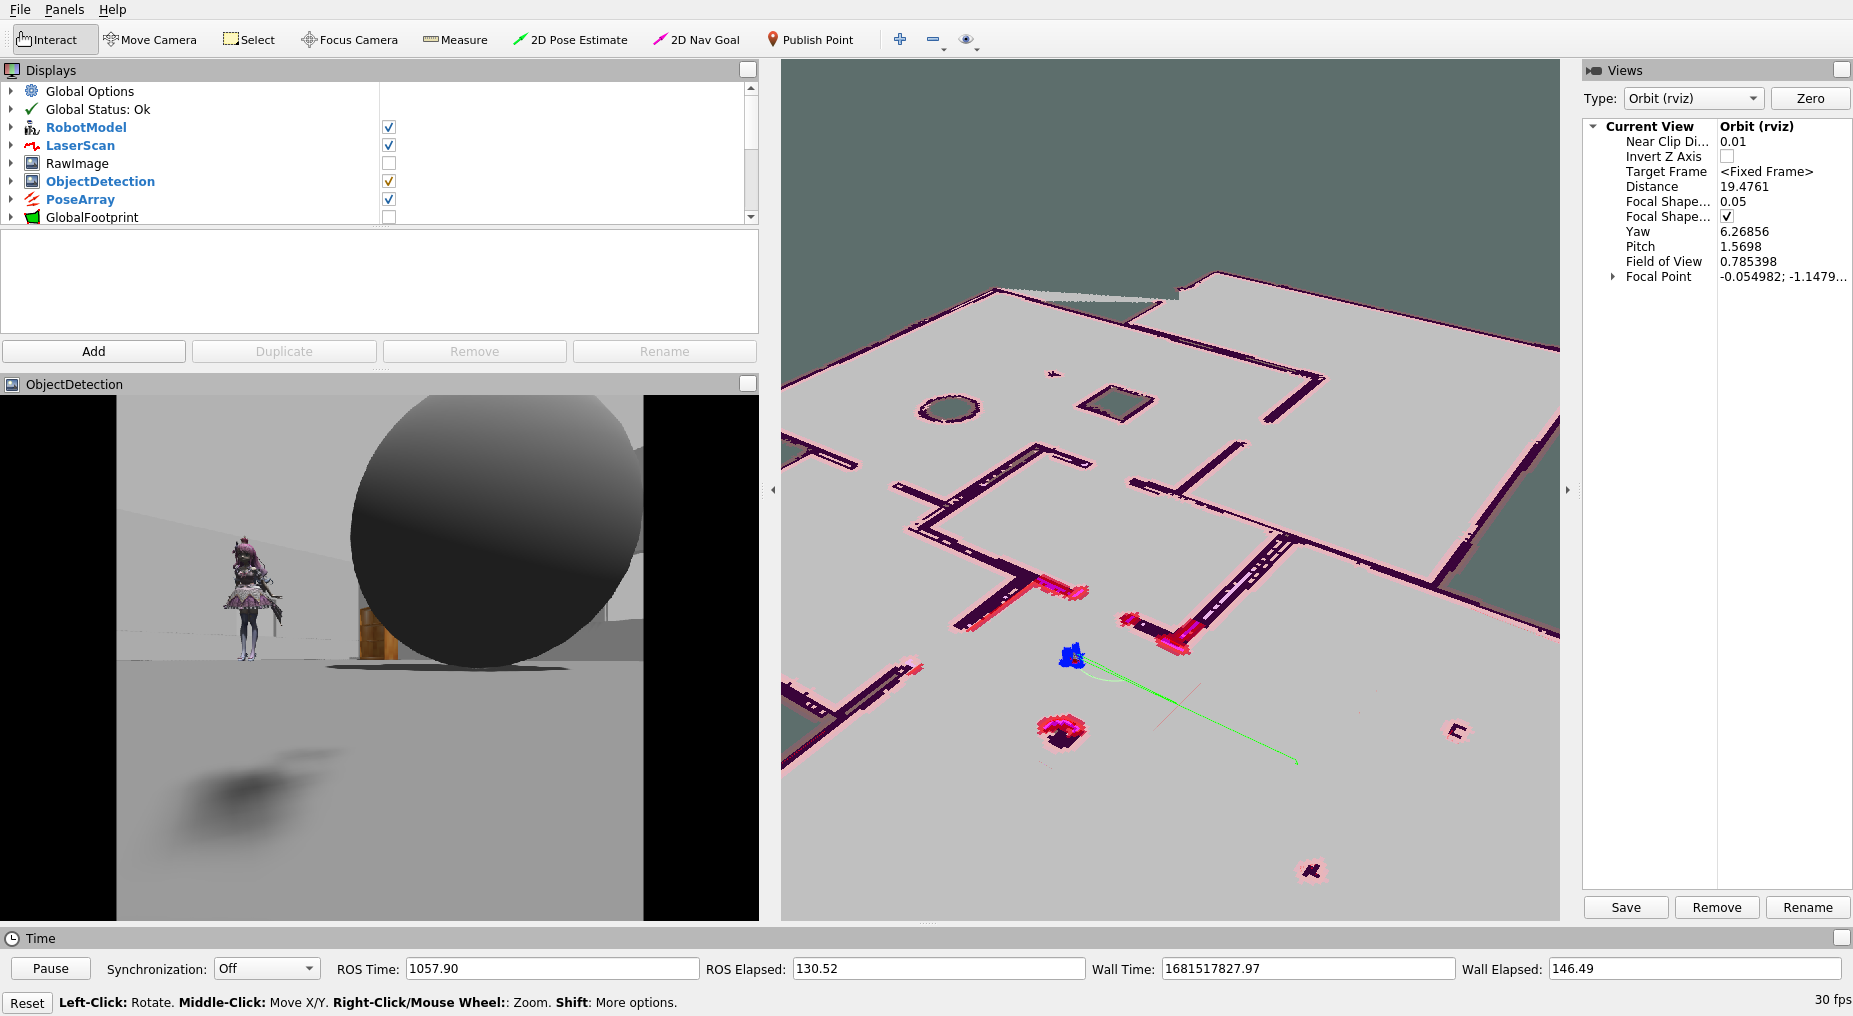
\includegraphics[width=\textwidth]{SLAM.png}
\caption{SLAM-based autonomous navigation in Gazebo Classic visualised with RViz.}
\label{fig:slam}
\end{figure}

Mapless navigation is a type of robotic task and refers to the ability of a robot to navigate its environment without relying on pre-built maps or prior knowledge of the environment. Instead, the system uses various sensors, such as cameras, LiDAR, or other depth sensors, to perceive its surroundings in real-time and plan the motion. This ability is particularly useful in situations where maps are unavailable, outdated, or impractical, such as in unpredictable terrains or rapidly changing environments.

The remainder of the report is organised as follows: Section \ref{sec:literature} surveys the literature related to DRL and mapless navigation. Section \ref{sec:impact} describes the value of this project from three perspectives. Section \ref{sec:theory} explains the theories used in this project. Section \ref{sec:design} presents the design. Section \ref{sec:method} focuses on the experimental method. Section \ref{sec:results} reports the results. Section \ref{sec:discussion} discusses the results and DRL. Section \ref{sec:reflection} reflects on this project-based learning. Finally, Section \ref{sec:conclusion} concludes the report.
